%//==============================--@--==============================//%
\subsection[5.1 Visão Geral]{\hspace*{0.075 em}\raisebox{0.2 em}{$\pmb{\drsh}$} Visão Geral}
\label{subsec:visao-geral}

\begin{theo}[\underline{Link Layer}]{def:Link-Layer}\label{def:Link-Layer}
    ``The basic service of any link layer is to move a datagram from one node to an adjacent node over a single communication link."\cite{Kurose2017}
\end{theo}

\noindent The link layer may provide the following services:
\begin{itemize}
    \item \textbf{Framing:} Encapsulates network-layer datagrams in link-layer frames. A frame consists of a data field, in which the network-layer datagram is inserted, and a number of header fields.
    \item \textbf{Link access:} MAC (Medium Access Control) protocol governs frame transmission, coordinating multiple nodes on a broadcast link.
    \item \textbf{Reliable delivery:} Ensures error-free transmission across the link, useful for high-error-rate links but unnecessary for low-error-rate links.
    \item \textbf{Error detection and correction:} Identifies and corrects bit errors introduced by signal attenuation and electromagnetic noise.
\end{itemize}

\noindent The link layer implementation:
\begin{itemize}
    \item Involves both hardware and software components.
    \item Uses a \textbf{network adapter}, also known as a \textbf{network interface controller (NIC)} for hardware implementation.
    \item Can be integrated into the motherboard chipset or implemented via a dedicated Ethernet chip.
    \item Handles various link layer services including framing, link access, and error detection.
\end{itemize}

\begin{figure}[H]
    \centering
    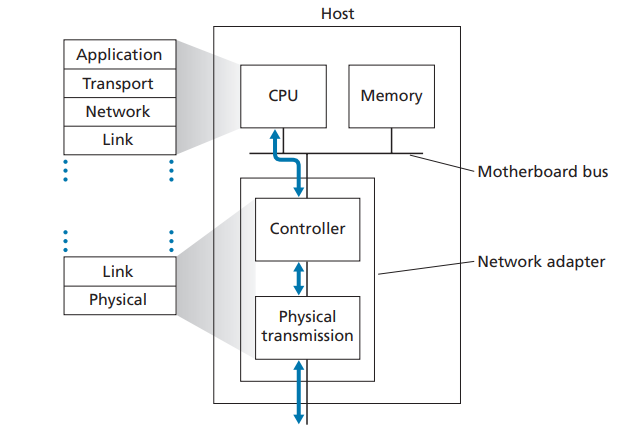
\includegraphics[width = 0.75\linewidth]{img/5/network-adapter.png}
    \caption{``Network adapter: relationship to other host components and to protocol stack functionality''\cite{Kurose2017}}
    \label{fig:network-adapter}
\end{figure}

\newpage
\noindent The link layer in the protocol stack involves both hardware and software components:
\begin{itemize}
    \item On the sending side:
    \begin{itemize}[nolistsep, noitemsep]
        \item The network adapter takes a datagram created and stored in host memory by higher layers of the protocol stack.
        \item It encapsulates the datagram in a link-layer frame.
        \item The frame is transmitted into the communication link following the link-access protocol.
    \end{itemize}
    \item On the receiving side:
    \begin{itemize}[nolistsep, noitemsep]
        \item The network adapter receives the entire frame.
        \item It extracts the network-layer datagram.
        \item Error detection is performed, if necessary.
    \end{itemize}
    \item Higher-level link-layer features are implemented in software running on the host's CPU:
    \begin{itemize}[nolistsep, noitemsep]
        \item Software components assemble link-layer addressing information.
        \item They activate the controller hardware.
        \item Error conditions are handled, and datagrams are passed up to the network layer.
    \end{itemize}
\end{itemize}

%//==============================--@--==============================//%